\documentclass[a4paper]{article}  
\usepackage[UTF8]{ctex}
\usepackage{xcolor}
\usepackage{graphicx}
\usepackage{geometry}
\usepackage{listings}
\usepackage{amsmath}
\usepackage{indentfirst}
\usepackage{subcaption}
\usepackage{hyperref}
\geometry{left=2.5cm,right=2.5cm,top=2.5cm,bottom=2.5cm}
\hypersetup{
colorlinks=true,
linkcolor=black
}
  
\begin{document} 

\begin{titlepage}  
    \centering  
    \huge \textbf{《系统开发工具基础》实验报告} \\  
      \vspace{5cm}  
    
     \begin{figure}[ht]
    \centering
    \includegraphics[width=0.5\textwidth]{pic/R-C.jpg}
\end{figure}
 \vspace{3cm} 
 
    \Large  
    \begin{tabular}{ll} 
        \textbf{题目:}&git和latex学习报告\\
        \cline{2-2} 
        \textbf{学号:} & 23020007139 \\ 
       \cline{2-2} 
        \textbf{姓名:} & 闫枳冰 \\  
        \cline{2-2} 
        \textbf{专业:} & 计算机科学与技术 \\  
       \cline{2-2} 
    \end{tabular}  
    \vspace{2cm}  
 
    \Large 日期: \today  
    
\end{titlepage}  
  
\pagenumbering{roman}
\tableofcontents
\newpage
\pagenumbering{arabic}

\section{实验目的}  
1.了解学习版本控制Git;

2.了解学习Latex文本编辑;
\section{实验内容及步骤}
\subsection{实验主要内容}
1.学习了Git的主要作用、工作原理、基本操作、如何克隆仓库以及关联本地仓库和远程仓库。\\

2.学习了如何用LaTeX编写文档以及一些基本的处理。
\subsection{实验具体步骤}
\subsubsection{git}
%加个git简介
1.下载安装git。
\begin{figure}[h] 
    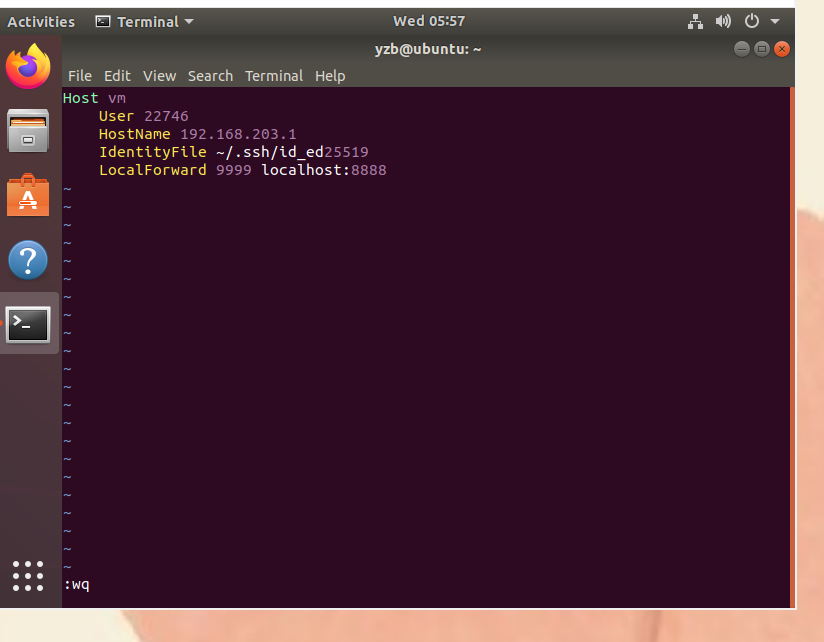
\includegraphics[width=0.18\textwidth]{pic/1.pdf}
     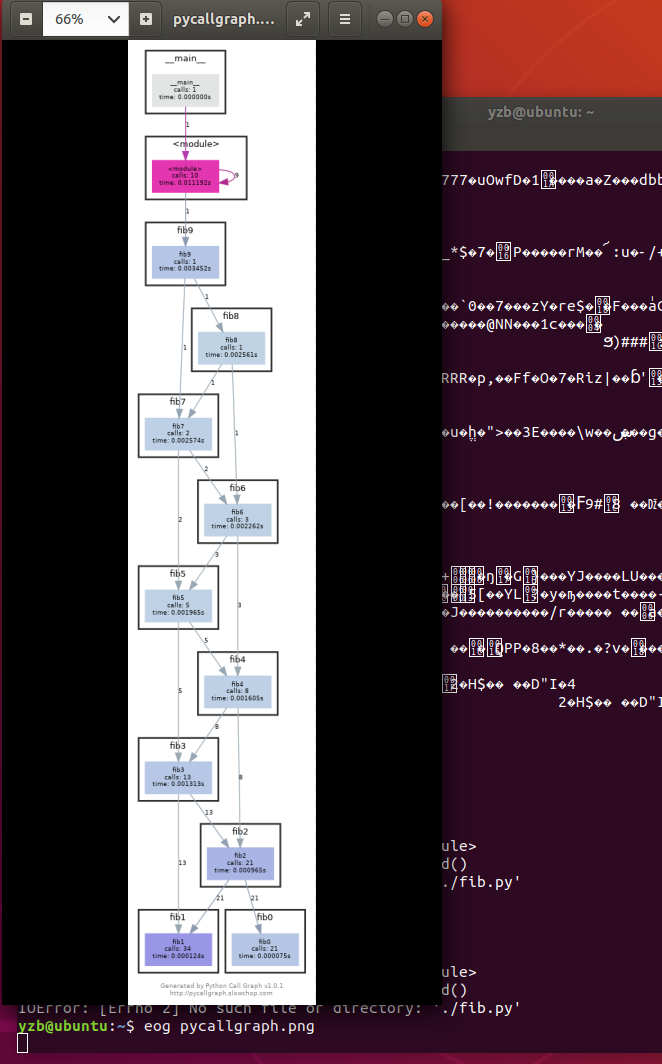
\includegraphics[width=0.18\textwidth]{pic/2.pdf}
     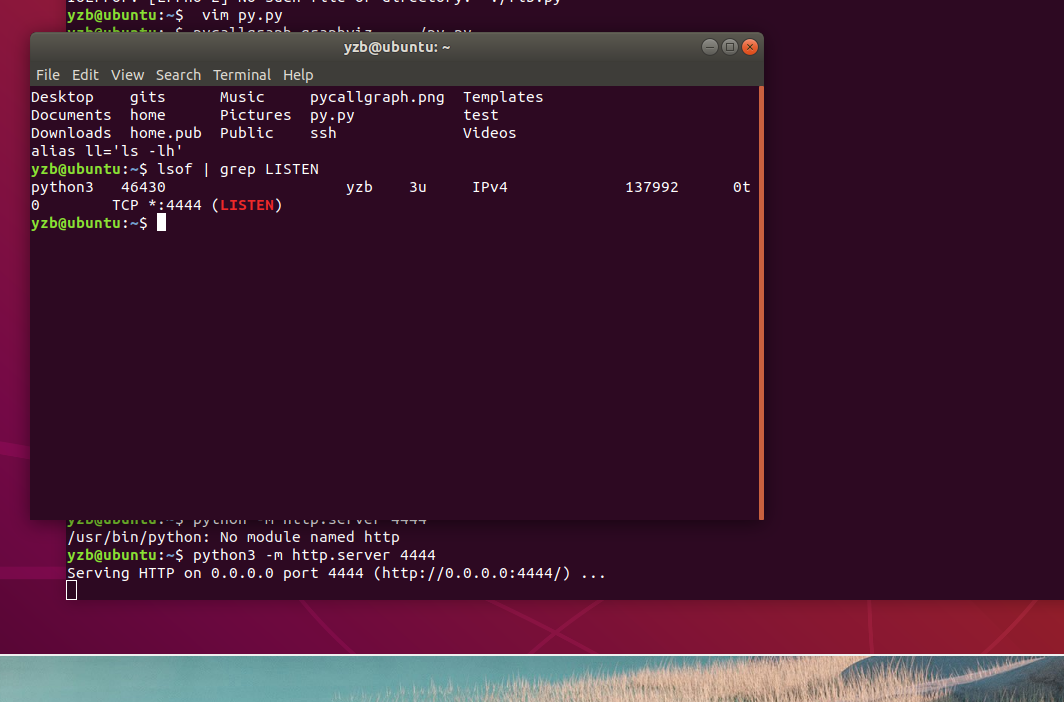
\includegraphics[width=0.18\textwidth]{pic/3.pdf}
      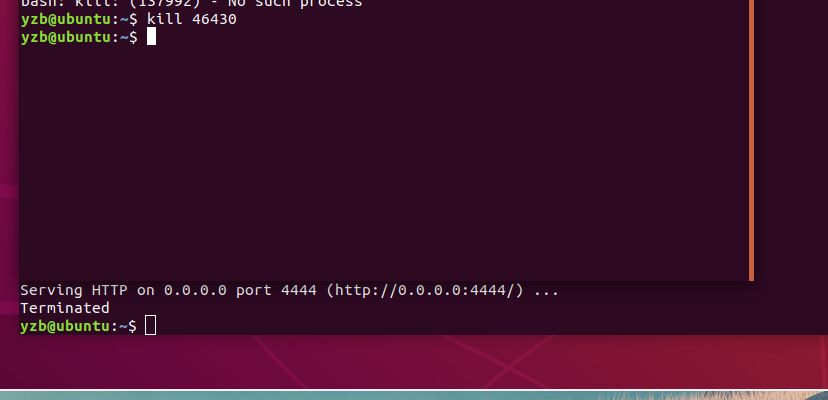
\includegraphics[width=0.18\textwidth]{pic/4.pdf}
       \includegraphics[width=0.18\textwidth]{pic/5.pdf}
    \includegraphics[width=0.18\textwidth]{pic/6.pdf}
    \includegraphics[width=0.18\textwidth]{pic/7.pdf}
     \includegraphics[width=0.18\textwidth]{pic/8.pdf}
    \includegraphics[width=0.18\textwidth]{pic/9.pdf}
    \includegraphics[width=0.19\textwidth]{pic/10.pdf}
    
\end{figure} 
\hfill

2.初始化配置。

首先如图1用“git config --global user.name "name"”初始化姓名;再图2用“git config --global user.name "email”初始化邮箱;再如图3输入“git config -l”和打开.gitconfig配置文件检查.

\begin{figure}[h] 
\centering
    \includegraphics[width=0.18\textwidth]{pic/2.1.jpg}
    \caption{姓名}
    \includegraphics[width=0.18\textwidth]{pic/2.2.jpg}
    \caption{邮箱}
    \includegraphics[width=0.18\textwidth]{pic/2.3.jpg}
    \includegraphics[width=0.18\textwidth]{pic/2.4.jpg}
    \caption{配置文件检查}
\end{figure} 
\vspace{2cm}
3.登录GitHub并配置SSH。

为了确保提交是本人,不是别人冒充,需要SSH Key。

首先在git Bash中执行ssh-keygen -t rsa ,来生成SSH Key,  
再如图四用 

cat \~/.ssh/id\_rsa.pub  
命令来查看生成的SSH公钥如图\ref{远程},并将其添加到GitHub的设置中。最后如图\ref{检查配置}输入检查配置是否成功。
\begin{figure}[h]
    \centering
    \includegraphics[width=0.5\linewidth]{远程.png}
    \caption{远程}
    \label{远程}
\end{figure}
\begin{figure}[h]
    \centering
    \includegraphics[width=0.18\textwidth]{pic/3.1.jpg}
\caption{查看ssh}
    \includegraphics[width=0.18\textwidth]{检查配置.png}
    \caption{检查配置}
    \label{检查配置}
\end{figure}

4.git的相关使用。

见3实例。
\subsubsection{latex}
latex的基本介绍:latex是一种语言工具,只用键盘就可以完成文档的排版和撰写,它分离了文档的内容和样式,有强大的公学公式排版能力和标准化复刻能力;也确保了文档的一致性,更容易维护。overleaf是latex的在线编排网站。

步骤:首先打开overleaf网站,注册登录;点击“New Project”,再点击“Blank Project”输入标题创建项目;最左侧是用来创建和管理文件,中间是用来编码,最右侧是查看编排的效果。

首先如图\ref{overleaf1}输入代码
\begin{figure*}[!h]
    \centering
    \includegraphics[width=0.18\textwidth]{pic/4.1.jpg}\caption{overleaf1}\label{overleaf1}
\end{figure*}
,其中第一行为声明文档类型,[]中输入字号,纸张类型,{}中输入文本类型;第二三行为宏包以扩展更多内容。正文部分放在代码段第五行和第七行中间。

在latex中用环境对命令进行包裹,让文本能有特殊格式或进行标识,如图\ref{overleaf2}。
\begin{figure*}[h]
 \centering
    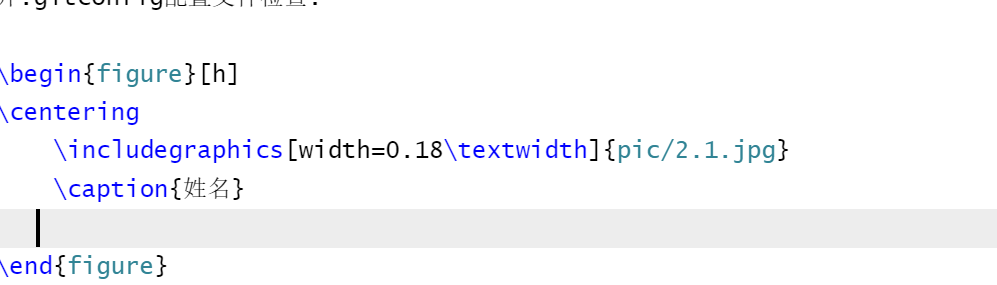
\includegraphics[width=0.18\textwidth]{pic/屏幕截图 2024-08-28 144705.jpg}\caption{overleaf2}\label{overleaf2}
\end{figure*}

编写实验报告模板需要对报告进行划分层次,可以对应命令及进行划分为摘要、部分、子部分、子子部分、附录、参考文献等。如图\ref{overleaf3}。
\begin{figure*}[!htb]
 \centering
    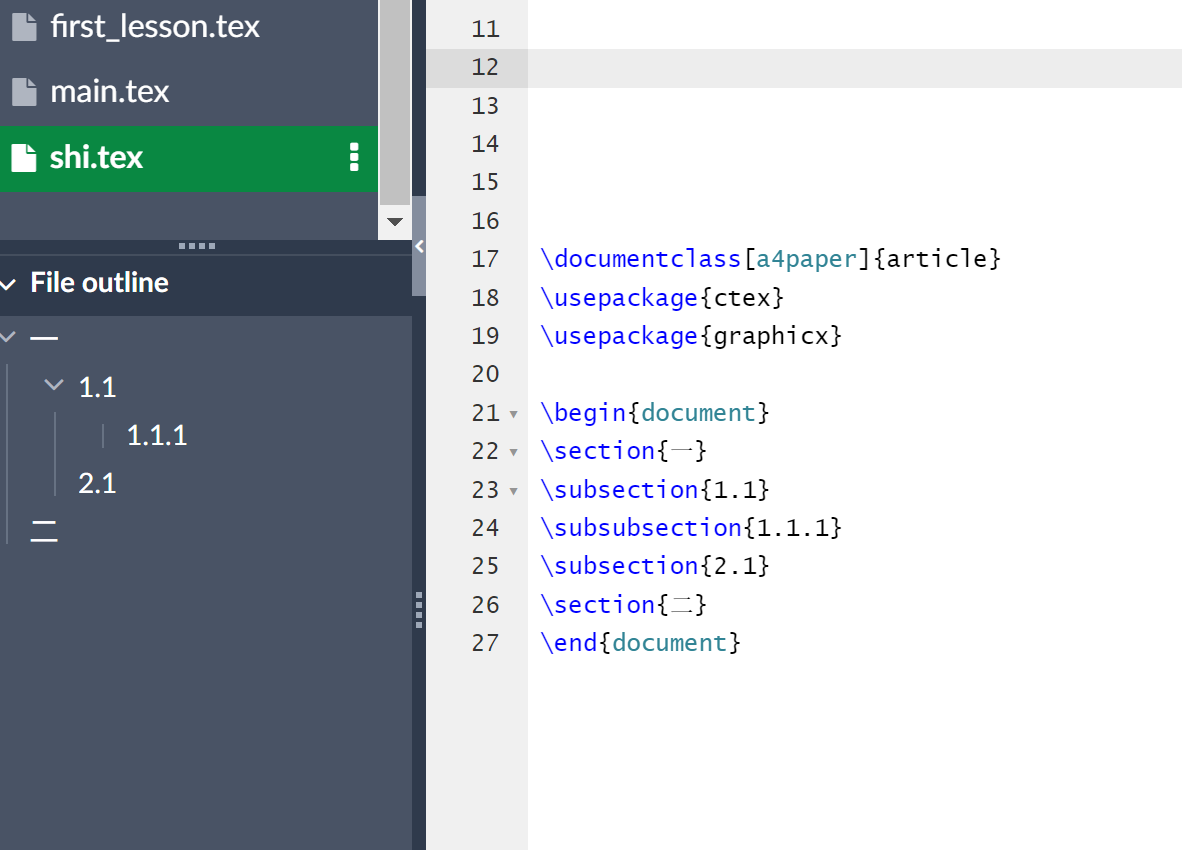
\includegraphics[width=0.18\textwidth]{pic/屏幕截图 2024-08-28 145435.png}\caption{overleaf3}\label{overleaf3}
\end{figure*}

此外,还需要其他具体操作和问题见3.实例
\subsection{练习记录}
链接:\href{https://github.com/yyy0202/-remote-repo/tree/main/%E7%AC%AC%E4%B8%80%E8%8A%82%E8%AF%BE/%E7%BB%83%E4%B9%A0%E8%AE%B0%E5%BD%95}{练习记录}

\section{实例}
\subsection{关于git的实例}
    \subsubsection{实例一:克隆课程网站的仓库。}
    
   使用git clone +远程仓库URL命令克隆,具体如图\ref{克隆仓库}和\ref{克隆仓库2}。
 \begin{figure*}[!h]
 \centering
    \includegraphics[width=0.23\textwidth]{pic/克隆仓库2.jpg}\caption{克隆仓库2}\label{克隆仓库2}
    \includegraphics[width=0.4\textwidth]{pic/克隆仓库.jpg}
    \caption{克隆仓库}
    \label{克隆仓库}
    \end{figure*}
    
查看仓库检查是否克隆成功,如图\ref{look}。
\begin{figure*}[htb!]
 \centering
    \includegraphics[width=0.15\textwidth]{pic/查看克隆仓库.jpg}
    \caption{查看克隆仓库}
    \label{look}
\end{figure*}

\vspace{1em} 


     \subsubsection{实例二:将版本历史可视化并进行探索}

方法一:在命令行中输入gitk。gitk提供了一个交互式的界面,可以浏览提交历史,查看差异,搜索特定的提交。如图\ref{gitk}。


\begin{figure*}[!htb]
 \centering
    \includegraphics[width=0.15\textwidth]{pic/gitk.jpg}\caption{gitk}\label{gitk}
\end{figure*}

方法二:使用git log命令,后加各种选项来导出数据。如输入git log --graph命令。得到如\ref{log}。

\begin{figure*}[!h]
 \centering
    \includegraphics[width=0.15\textwidth]{pic/5.1.jpg}\caption{log}\label{log}
\end{figure*}

\vspace{1em} 

 \subsubsection{实例三:是谁最后修改了 \texttt{README.md} 文件?}

输入命令 git log --pretty=format:"\%an <\%ae>" -n 1 README.md

如图\ref{rename.md}就可以看到最后修改该文件的作者和邮箱。其中--pretty=format:""用于自定义git log的输出格式,\%an代表作者,\%an代表邮箱,-n 1代表最近的提交记录,最后加文件名。

\begin{figure*}[!ht]
\centering
    \includegraphics[width=0.15\textwidth]{pic/rename.png}\caption{git rename.md}\label{rename.md}
\end{figure*}

注意:只输入git log,最后提交的最先输出。

\vspace{1em} 


 \subsubsection{实例四:最后一次修改 \_config.yml 文件中 collections: 行时的提交信息是什么?}

首先进入输入cd 远程仓库{}进入"远程仓库”文件夹,然后输入git blame \_config.yml,找到包含 collections: 的行,并记下该行旁边的提交哈希值,如图为a88b4eac。再输入git show a88b4eac,得到提交信息为“Redo lectures as a collection”。具体如图\ref{git blame}和图\ref{git con}和图\ref{git show}所示。

\begin{figure*}[htb!]
\centering
    \includegraphics[width=0.18\textwidth]{pic/git blame.png}\caption{git blame}\label{git blame}
    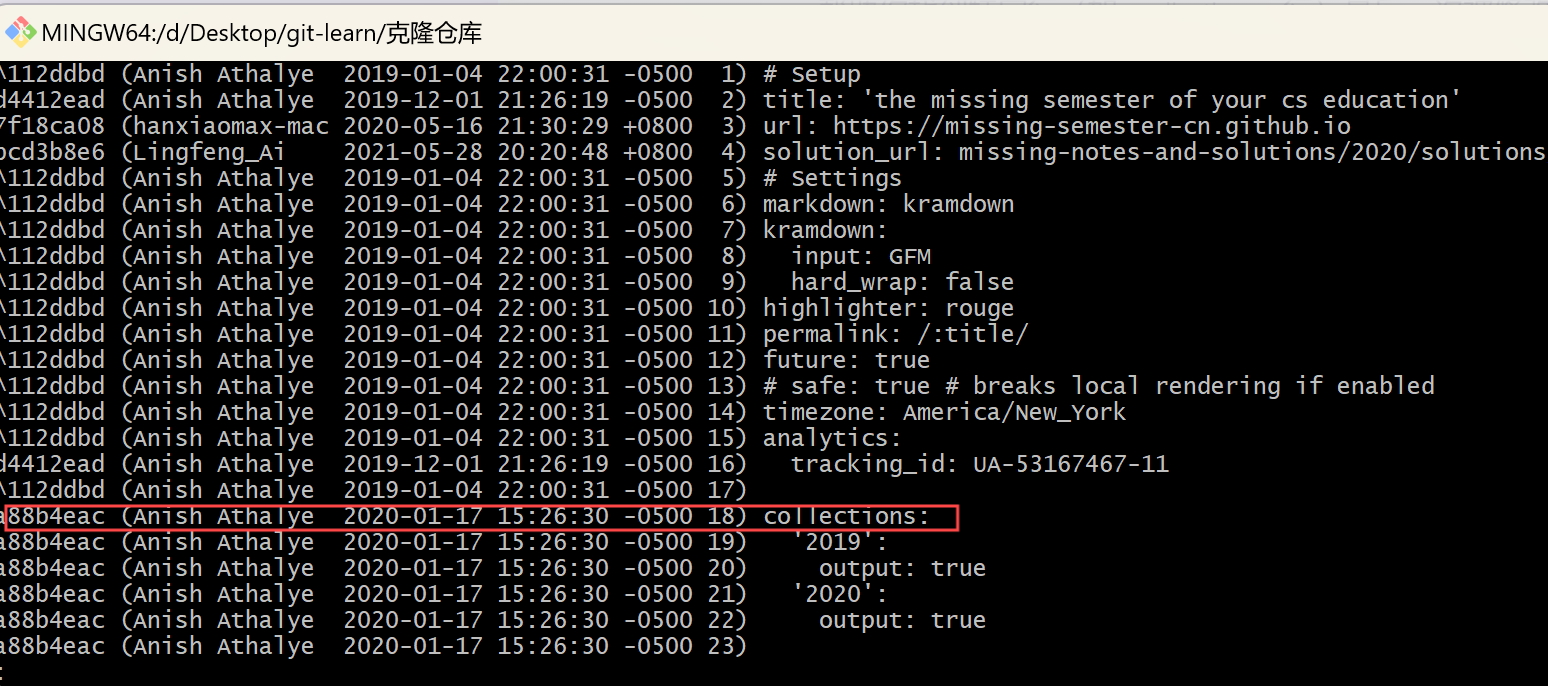
\includegraphics[width=0.18\textwidth]{pic/找到con.png}\caption{find}\label{git con}
    \includegraphics[width=0.18\textwidth]{pic/git show.jpg}\caption{git blame}\label{git show}
\end{figure*}

\vspace{1em} 


 \subsubsection{实例五:从 GitHub 上克隆某个仓库,修改一些文件。当您使用 git stash 会发生什么?当您执行 git log --all --oneline 时会显示什么?通过 git stash pop 命令来撤销 git stash 操作,什么时候会用到这一技巧?}

使用git stash会保存工作区和暂存区的更改,创建一个新的stash条目其中包含了当前工作目录和暂存区的所有更改;然后清理工作区和暂存区,被重置为它们最近的提交状态。


当执行git log --all --oneline时显示所有分支包括 stash的提交历史,如图\ref{12}。
\begin{figure*}[!htb]
    \centering
    \includegraphics[width=0.15\textwidth]{pic/git log --all --o.jpg}
    \caption{git log --all --oneline}
    \label{12}
\end{figure*}

执行git stash pop会恢复之前通过git stash保存的工作区和暂存区的更改,就再进行commit了,如图\ref{pop}。
\begin{figure*}[!htb]
    \centering
    \includegraphics[width=0.15\textwidth]{pic/git log --all --o2.jpg}
    \caption{git stash pop}
    \label{pop}
\end{figure*}

使用这一技巧的时候:当在一个分支上工作,但需要切换到另一个分支处理任务,但不想提交当前的更改,你可以使用git stash保存更改,然后切换分支。处理完紧急任务后,再切换回原来的分支并使用git stash pop恢复之前的工作;清理工作区进行其他任务,但又不想放弃当前的更改时,先git stash,处理完其他任务后再git stash pop回来;预计即将进行的合并或拉取操作可能会与当前更改发生冲突,可以先git stash这些更改,进行合并或拉取,然后再git stash pop它们回来。

\vspace{1em} 

 \subsubsection{实例六:关联本地仓库和远程仓库}

输入git remote add origin git@github.com:yyy0202/-remote-repo.git,在输入git remote -v查看是否关联成功,得到如图\ref{关联}所示,证明关联成功。再输入git push -u origin main将本地仓库更改推送到远程仓库。
\begin{figure*}[!htb]
    \centering
    \includegraphics[width=0.5\linewidth]{关联.png}
    \caption{关联远程仓库}
    \label{关联}
\end{figure*}

注意:如果远程仓库和本地仓库内容不一致,需要先输入git pull将内容统一。

\vspace{1em} 
\subsubsection{实例七:将文件上传到远程仓库}
将文件添加提交后,输入“git push origin 分支名”,文件被上传,如图\ref{上传}。
\begin{figure*}[!htb]
    \centering
    \includegraphics[width=0.5\linewidth]{上传.png}
    \caption{上传到远程仓库}
    \label{上传}
\end{figure*}
 \subsubsection{实例八:创建分支、切换分支、合并分支。}

分支同时能够进行多个功能开发,如果某个分支开发失败,也不会对其他分支造成影响。

输入git branch -v查看分支,如图\ref{branch1}所示,说明当前只有main。
\begin{figure*}[!htb]
    \centering
    \includegraphics[width=0.15\textwidth]{pic/branch2.png}
    \caption{git branch -v}
    \label{branch1}
\end{figure*}
再输入“git branch 分支名”命令,来创建分支,再进行查看,如图\ref{branch2},*在哪里表示当前在哪个分支。
\begin{figure*}[!htb]
    \centering
    \includegraphics[width=0.15\textwidth]{branch1.png}
    \caption{git branch}
    \label{branch2}
\end{figure*}

输入“git checkout 分支名”来切换分支,如图\ref{branch3}切换到branch1,对222.txt文档进行修改,添加提交后,查看提交记录,发现分支状态依然从工作区到暂存区再到仓库。
\begin{figure*}[!htb]
    \centering
    \includegraphics[width=0.15\textwidth]{branch3.png}
    \caption{branch checkout}
    \label{branch3}
\end{figure*}

输入“git merge 需要合并的分支名称”,如图\ref{branch4}在main分支中合并branch1分支,查看222.txt内容是最新在branch分支中修改的内容。注意:当合并冲突时,需要手动合并。
\begin{figure*}[!htb]
    \centering
    \includegraphics[width=0.15\textwidth]{branch4.png}
    \caption{branch merge}
    \label{branch4}
\end{figure*}[htb]

\vspace{1em}
 
\subsubsection{实例九:git diff的用法}
git diff能显示工作区、暂存区和本地仓库之间的差异;不同版本之间的差异;不同分支之间的差异。

1.工作区和暂存区之间的差异。输入"git diff"查看工作区和暂存区的差异,后加“--文件名”查看这个文件在工作区和暂存区的差异,输入“git diff -- 文件名1 文件名2”查看多个文件工作区和暂存区之间的差异。如图\ref{diff1}。
\begin{figure*}[!htb]
    \centering
    \includegraphics[width=0.15\textwidth]{image.png}
    \caption{git diff1}
    \label{diff1}
\end{figure*}

2.工作区和仓库之间的差异。输入“git diff HEAD”查看所有文件工作区和仓库之间的差异,后加“--文件名”查看这个文件在工作区和仓库的差异,输入“git diff HEAD -- 文件名1 文件名2”查看文件之间的差异。“git diff HEAD 具体版本 -- 文件名”查看工作区与具体某个版本之间的指定文件的差异。如图\ref{diff2}。
\begin{figure*}[!htb]
    \centering
    \includegraphics[width=0.15\textwidth]{diff2.png}
    \caption{git diff2}
    \label{diff2}
\end{figure*}

3.查看暂存区和版本库之间的差异。输入“git diff --cached”查看所有文件工作区和仓库之间的差异,后加“--文件名”查看这个文件在工作区和仓库的差异,输入“git diff --cached -- 文件名1 文件名2”查看文件之间的差异。“git diff --cached 具体版本 -- 文件名”查看工作区与具体某个版本之间的指定文件的差异。如图\ref{diff3}。
\begin{figure*}[!htb]
    \centering
    \includegraphics[width=0.2\textwidth]{diff3.png}
    \caption{git diff3}
    \label{diff3}
\end{figure*}

 4.查看不同版本库之间的差异。输入“git diff 版本号1 版本号2”。查看具体文件等,同1、2、3操作在后加“ -- 文件名”等。如图\ref{diff4}
\begin{figure*}[!htb]
    \centering
    \includegraphics[width=0.23\textwidth]{diff4.png}
    \caption{diff4}
    \label{diff4}
\end{figure*}

\subsubsection{实例十:在 ~/.gitconfig 中创建一个别名,使在运行 git graph 时,可以得到 git log --all --graph --decorate --oneline 的输出结果}

首先输入“vim \~/.gitconfig”打开配置文件,在其中输入“[alias]  
    graph = log --all --graph --decorate --oneline”,退出后输入git graph验证。如图\ref{config}
\begin{figure*}[!htb]
    \centering
    \includegraphics[width=0.5\linewidth]{config.png}
    \caption{gitconfig}
    \label{config}
\end{figure*}
\subsection{关于latex的实例}
\subsubsection{实例十一:让latex支持中文字体}

在文档开头添加\textbackslash{}usepackage\{xeCJK\}或者\textbackslash{}usepackage[UTF8]\{ctex\}宏包.

\subsubsection{实例十二:插入图片}
如图\ref{插入图片},输入图中代码块,成功插入图片。

\begin{figure*}[!htb]
    \centering
    \includegraphics[width=0.5\linewidth]{pic/插入图片.png}
    \caption{latex插入图片}
    \label{插入图片}
\end{figure*}

\subsubsection{实例十三:添加目录}
输入如下代码块,添加目录。如图\ref{t}。
\begin{figure*}[!h]
    \centering
    \includegraphics[width=0.5\linewidth]{添加目录.png}
    \caption{添加目录}
    \label{t}
\end{figure*}
\subsubsection{实例十四:绘制表格}
按照对应代码,如图\ref{表格},绘制了两个表格。一些常见的操作有\& 绘制分割列;
\textbackslash{}\textbackslash{} 用于换行;
\textbackslash{}hline 表示插入一个贯穿所有列的横着的分割线;
\textbackslash{}cline{1-2} 会在第一列和第二列插入一个横着的分割线。
\begin{figure*}[!htb]
    \centering
    \includegraphics[width=0.5\linewidth]{表格.png}
    \caption{表格}
    \label{表格}
\end{figure*}
\subsubsection{实例十五:特殊字符的转义,输出"Item \#A\textbackslash642 costs \$8 \& is sold at a \^{}10\% profit."字符串}

如图,输出。其中\# \$ \% \^{} \& \_ \{ \} \~{}需要在前面加反斜杠。\^{}需要在后面加\~{},否则会变成\^10。反斜杠使用 \textbackslash{}textbackslash 命令代替。
\begin{figure*}[!h]
    \centering
    \includegraphics[width=0.5\linewidth]{特殊.png}
    \caption{特殊字符}
    \label{特殊字符}
\end{figure*}

\subsubsection{实例十六:字体颜色、大小、效果}
在文档前加\textbackslash{}usepackage{color}宏包,按照对应格式输出。如图\ref{效果}。
\begin{figure*}[!h]
    \centering
    \includegraphics[width=0.5\linewidth]{字效果.png}
    \caption{字效果、大小、颜色}
    \label{效果}
\end{figure*}
\subsubsection{实例十七:攥写公式}

题目:输出如下
\begin{eqnarray}
     e&=&mc^2 \\
     \pi&=&\frac{c}{d}\\
     \frac{d}{dx}\int_0^{\infty} f(s)ds&=&f(s)\\
     f(x)&=&\sum_{i} 0^{\infty}\frac{f^{(i)}(0)}{i!}x^i \\
     x&=&\sqrt{\frac{x_i}{z}y}
\end{eqnarray}

代码块如图\ref{公式}:
\begin{figure*}[!h]
    \centering
    \includegraphics[width=0.5\linewidth]{公式.png}
    \caption{公式}
    \label{公式}
\end{figure*}

\subsubsection{实例十八:创建列表}
创建如下列表:
\begin{enumerate}
  \item First 
  \item Second 
\begin{itemize}
      \item second-first

      \item second-second
 \end{itemize}

  \item Third
\end{enumerate}
代码如图\ref{列表}:
\begin{figure*}[!h]
    \centering
    \includegraphics[width=0.5\linewidth]{列表.png}
    \caption{列表}
    \label{列表}
\end{figure*}
\subsubsection{实例十九:插入代码块}
\lstset{
 columns=fixed,       
 numbers=left,                                       
 numberstyle=\tiny\color{gray},                      
 frame=none,                                         
 backgroundcolor=\color[RGB]{245,245,244},           
 keywordstyle=\color{blue},    
 stringstyle=\rmfamily\color[RGB]{128,0,0},
 language=c++,                                      
}
\begin{lstlisting}

#include <iostream>
using namespace std;

int main()
{
    cout<<"hello"<<endl;
    return 0;
}
\end{lstlisting}

代码如图\ref{代码}
    \begin{figure*}[!htb]
        \centering
        \includegraphics[width=0.3\linewidth]{代码.png}
        \caption{代码}
        \label{代码}
    \end{figure*}

\subsubsection{实例二十:标题等级}
如图\ref{标题等级},可以划分标题等级。
\begin{figure*}[!htb]
    \centering
    \includegraphics[width=0.3\linewidth]{标题等级.png}
    \caption{标题等级}
    \label{标题等级}
\end{figure*}
\section{实验结果}
\subsection{关于git}
了解学习了git的基本命令行和操作,创建了自己的远程仓库并与本地仓库关联用于上传作业。
github链接:\href{https://github.com/yyy0202/-remote-repo.git}{https://github.com/yyy0202/-remote-repo.git}
\subsection{关于latex}
了解学习了latex的基本操作并进行练习,创建了自己实验报告的模板并编写了实验报告。图\ref{模板}和\ref{模板2}
\begin{figure*}[!h]
    \centering
    \includegraphics[width=0.5\linewidth]{模板1.png}
    \caption{模板}
    \label{模板}
\end{figure*}
\begin{figure*}[!h]
    \centering
    \includegraphics[width=0.5\linewidth]{模板2.png}
    \caption{模板}
    \label{模板2}
\end{figure*}
\section{解题感悟}
\subsection{学习git的感悟}
git在学习之初,可能会觉得git的命令行操作复杂,但随着越来越熟练,就能体会到它的便利和高效。尤其是git通过创建分支、提交记录等能够为团队协作提供便利,多人协作中的冲突能够被解决等,在学习过程中,我也遇到了很多问题,比如git pull不成功、修改文件名后git对同一个文件追踪两次等,这需要去不断探索和学习来解决问题。
\subsection{学习latex的感悟}
刚开始学习latex,会觉得有点复杂总是报错,不如word好用。但随着学习,我体会到了latex的方便。比如说可以通过几行代码自动生成目录,可以很快的写出美观的数学公式、表格等。在学习过程中我也遇到了很多困难,比如插入的图片都在最后一页,首段没有空两格等。但通过练习和总结,提高了我的latex使用能力。

\end{document}
